\documentclass[tikz,border=7pt]{standalone}
\usepackage{amsmath}
\usepackage[T1]{fontenc}
\usetikzlibrary{positioning,arrows.meta}
\tikzset{box/.style={draw,rectangle,rounded corners=2pt,minimum width=70mm,minimum height=38mm,align=left},arr/.style={-{Latex[length=2mm]},thick}}
\begin{document}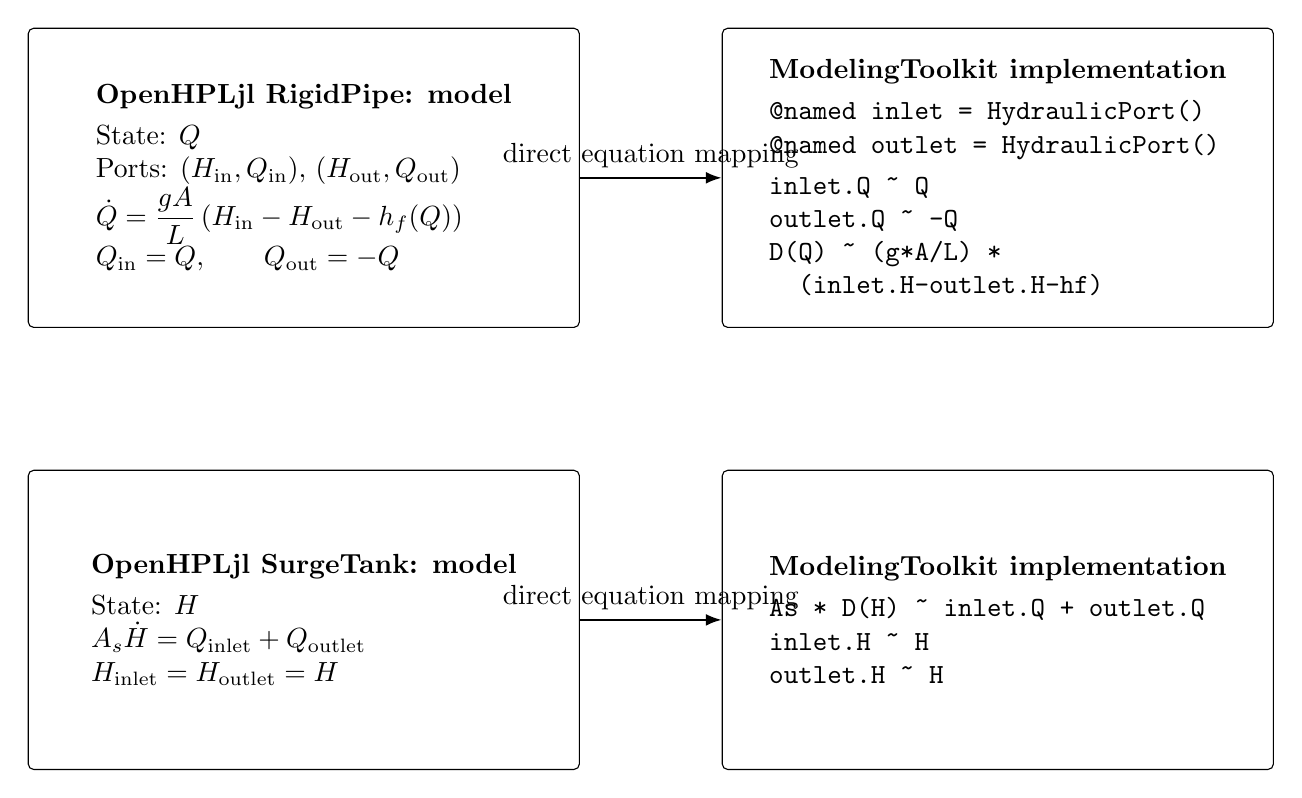
\begin{tikzpicture}[node distance=18mm]
\node[box] (physics) {\textbf{OpenHPLjl RigidPipe: model}\\[1mm]
State: $Q$\\
Ports: $(H_{\rm in},Q_{\rm in})$, $(H_{\rm out},Q_{\rm out})$\\
$\displaystyle \dot Q=\frac{gA}{L}\left(H_{\rm in}-H_{\rm out}-h_f(Q)\right)$\\
$\displaystyle Q_{\rm in}=Q,\qquad Q_{\rm out}=-Q$};
\node[box,right=of physics] (code) {\textbf{ModelingToolkit implementation}\\[1mm]
\texttt{@named inlet = HydraulicPort()}\\
\texttt{@named outlet = HydraulicPort()}\\[1mm]
\texttt{inlet.Q \string~ Q}\\
\texttt{outlet.Q \string~ -Q}\\
\texttt{D(Q) \string~ (g*A/L) *}\\
\texttt{\ \ (inlet.H-outlet.H-hf)}};
\draw[arr] (physics) -- node[above] {direct equation mapping} (code);
\node[box,below=of physics] (surge) {\textbf{OpenHPLjl SurgeTank: model}\\[1mm]
State: $H$\\
$\displaystyle A_s\dot H=Q_{\rm inlet}+Q_{\rm outlet}$\\
$\displaystyle H_{\rm inlet}=H_{\rm outlet}=H$};
\node[box,right=of surge] (surgecode) {\textbf{ModelingToolkit implementation}\\[1mm]
\texttt{As * D(H) \string~ inlet.Q + outlet.Q}\\
\texttt{inlet.H \string~ H}\\
\texttt{outlet.H \string~ H}};
\draw[arr] (surge) -- node[above] {direct equation mapping} (surgecode);
\end{tikzpicture}\end{document}
